% ch13-systems.tex -- Concurrency and synchronisation
\chapter{Concurrency and synchronisation}
\label{ch:systems13}
\index{race condition}\index{mutex}\index{condition variable}\index{deadlock}

Imagine two cooks sharing one recipe card, and the card says
``eggs used: 5''. Cook one reads 5, goes to fetch an egg, and writes
6. Meanwhile cook two also read 5 before cook one wrote anything, and
also writes 6. Two eggs were used; the card says one. Nobody did
anything wrong step by step, and the card is still wrong. That is
the whole problem of this chapter, and it is the reason programs
with several threads are famous for bugs that appear only on some
runs. Chapter~\ref{ch:systems12} gave every process its own world;
here threads share one world, and we watch it break, then learn
the tools that keep it intact, and price each tool on a real
machine.

\begin{wins}[What you will be able to do]
After this chapter you can write a small multi-threaded C program,
make it lose updates on purpose, and then fix it in three different
ways. You can build a producer and consumer that wait for each other
correctly with a condition variable, show the classic
\texttt{if}-instead-of-\texttt{while} bug in action, and turn a
deadlock into a visible, repeatable report and cure it with a lock
order. You will also know how to read a scaling curve without
trusting it blindly, including spotting the case where the compiler
quietly deleted the work you meant to time.
\end{wins}

\begin{rulebox}[Before you start]
A \emph{thread} is a separate line of execution inside one process:
threads share the same memory but each has its own registers and
stack (the process, from ch.~\ref{ch:systems12}, is the house; threads
are the people living in it). The hardware underneath is what Book~7
ch.~\ref{ch:systems10} (caches) showed: memory is moved in 64-byte
\emph{cache lines}, and a core that writes a line must own it. If you
want a reminder of how registers and a bus move one value at a time,
Book~5 ch.~15 (registers, buses and the datapath) is that picture
in hardware.

\emph{A short C refresher.} \texttt{pthread\_create(\&t, 0, f, arg)}
starts function \texttt{f(arg)} as a new thread and stores its handle
in \texttt{t}; \texttt{pthread\_join(t, 0)} waits for it to finish.
A \texttt{static} global variable is visible to every thread.
\texttt{volatile} tells the compiler ``this value may change behind
your back, really read and write it every time''. \texttt{counter++}
is shorthand for three steps: load, add one, store. Compile with
\texttt{gcc -O2 -pthread file.c}. Numbers marked \emph{Mac} come from
the author's earlier laptop; numbers marked \emph{Linux} come from a
4-vCPU Intel Xeon container (2.8\,GHz, gcc 13) and are kept apart.
\end{rulebox}

\begin{principle}[Think like this]
For any shared value, ask three questions in order. Who else can touch
it? What \emph{sequence} of steps must be indivisible? What is the
cheapest way to make that sequence indivisible, or to stop sharing the
value at all? The best answer in this chapter is almost always the
last one.
\end{principle}

\begin{principle}[Concept: critical section and invariant]
A \emph{critical section} is a stretch of code that must run as if
nobody else were running at the same time. Why must it? Because
while the code is half done, some fact about the data is
temporarily false. For the egg card the fact is ``the number on the
card equals the eggs used''; between ``read 5'' and ``write 6'' it is
false for a moment. Such a fact is an \emph{invariant}. The skilled
habit is to name the invariant first, then find the smallest piece of
code during which it is broken, and protect exactly that piece. Too
large a critical section makes threads wait for no reason (slow);
too small leaves the invariant exposed (wrong).
\end{principle}

\section{The race, demonstrated}
\label{sec:race13}

\begin{figure}[htbp]
\centering
\begin{tabular}{lll}
\toprule
$T_1$ (counter++) & $T_2$ (counter++) & counter \\
\midrule
load c (=5)  &              & 5 \\
             & load c (=5)  & 5 \\
$t{+}1$, store (6) &      & 6 \\
             & $t{+}1$, store (6) & \textbf{6} \\
\bottomrule
\end{tabular}
\caption{Two threads, one increment each, one lost. Both loaded 5,
both wrote 6 --- the interleaving throws away an entire update.
Run for real: 6 threads lost 2\,480\,483 of 3\,000\,000 updates
(83\%) on the Mac.}
\label{fig:racetime13}
\end{figure}


\begin{example}[83\% of updates lost, real (Mac)]
\texttt{ch13\_race.c} runs 6 threads of the unprotected
\texttt{load--add--store} sequence, 500\,k increments each. Three
runs: counter lands at 519\,517, 502\,923, 521\,101 --- never the
expected 3\,000\,000. Each run loses $\approx$2.5\,million updates
because both threads load before either stores. A race isn't a
sometimes-bug; under contention it is the \emph{usual} result.
\end{example}

\begin{example}[The same race on the Linux container]
\emph{What we expected.} The same 83\% loss. \emph{What happened.}
Five runs of the same program gave very different answers, as the
listing shows. The lesson is that the loss rate is not a constant of
the program: it depends on how often two threads happen to overlap in
the tiny load--store window, which depends on the machine, the
number of cores and the moment.

\begin{lstlisting}[language=C,basicstyle=\ttfamily\scriptsize,caption={The racy
loop from \texttt{ch13\_race.c}, and real output of five runs of
the compiled program (Linux x86\_64 container, \texttt{gcc -O2}).}]
static volatile long counter;                   // shared by all 6 threads
for (long i = 0; i < 500000; i++) { long t = counter; t = t + 1; counter = t; }

counter=1594598 (expected 3000000, lost 1405402)
counter=2062530 (expected 3000000, lost 937470)
counter=501840 (expected 3000000, lost 2498160)
counter=2113490 (expected 3000000, lost 886510)
counter=2142752 (expected 3000000, lost 857248)
\end{lstlisting}
Lost fractions: $1405402/3000000=47\%$, $31\%$, $83\%$, $30\%$,
$29\%$. Building with \texttt{-O0} changed nothing important (three
runs lost 1.38\,M, 2.01\,M and 1.91\,M). The point to carry away: a
program that is wrong in one run and ``almost right'' in another is
not partly correct, it is incorrect, and testing alone will not tell
you which kind of run you got.
\end{example}

\section{The atomic ladder}
\label{sec:atomic13}

\begin{figure}[htbp]
\centering
\begin{tabular}{ll}
\toprule
mechanism & the atomic unit it gives you \\
\midrule
\texttt{lr.d}/\texttt{sc.d} (RISC-V A) & load-reserved + store-conditional retry loop \\
\texttt{amoadd} (RISC-V A) & atomic memory op, no retry \\
C11 \texttt{atomic\_fetch\_add} & portable; compiles to the above \\
\texttt{pthread\_mutex} & sleep-lock over the same primitives \\
\bottomrule
\end{tabular}
\caption{The atomic ladder. Everything in this chapter stands on
the hardware's indivisible read-modify-write; locks are policy built
on top of it.}
\label{fig:atomic13}
\end{figure}


Why can a fix not be ``just write the code more carefully''? Because
the problem lives between instructions, where the program cannot
see. The only way out is help from the hardware.
Hardware provides one indivisible thing: a read-modify-write that
no other core can interleave with. RISC-V's A extension gives two
flavours --- \texttt{lr.w}/\texttt{sc.w} (load-reserved /
store-conditional, the retry-loop primitive; \texttt{.d} on RV64) and
\texttt{amo} instructions (atomic memory ops that complete without a retry).
Every synchronisation primitive above them is software.

\section{Three fixes, one measurement}
\label{sec:fix13}

Same race, fixed three ways: a mutex around the increment, a C11
\texttt{atomic\_fetch\_add}, and partitioning (each thread counts
privately, sum at the end). \texttt{ch13\_lockscale.c} times all
three at 1--8 threads:

\begin{figure}[htbp]
\centering
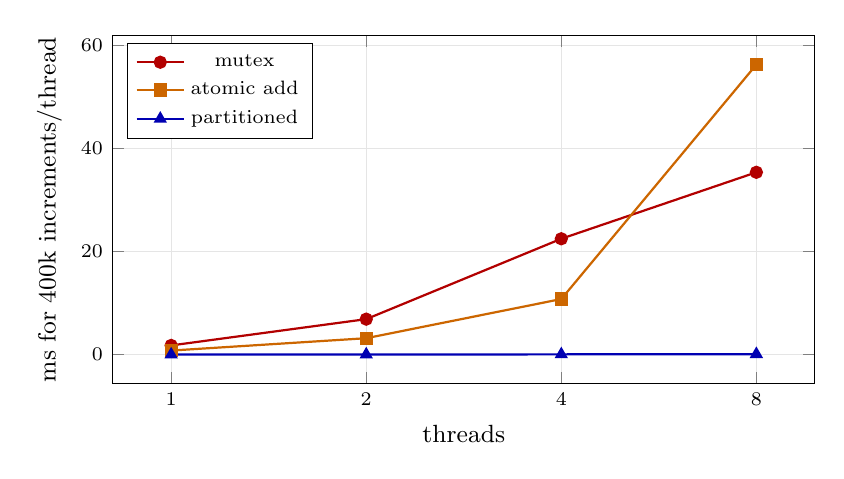
\begin{tikzpicture}
\begin{axis}[width=10.5cm,height=6cm,
  xlabel={threads}, ylabel={ms for 400k increments/thread},
  symbolic x coords={1,2,4,8}, xtick=data,
  grid=major, grid style={gray!20},
  tick label style={font=\scriptsize}, label style={font=\small},
  legend style={font=\scriptsize, at={(0.02,0.98)}, anchor=north west}]
\addplot[thick,mark=*,color=red!70!black] coordinates {(1,1.8)(2,6.9)(4,22.5)(8,35.4)};
\addplot[thick,mark=square*,color=orange!80!black] coordinates {(1,0.8)(2,3.2)(4,10.8)(8,56.3)};
\addplot[thick,mark=triangle*,color=blue!70!black] coordinates {(1,0.031)(2,0.032)(4,0.065)(8,0.109)};
\legend{mutex, atomic add, partitioned}
\end{axis}
\end{tikzpicture}
\caption{Real \texttt{ch13\_lockscale.c} on this laptop. Partitioning
is flat ($\sim$0.1\,ms) because nothing is shared. The honest
surprise: at 8 threads the atomic add is \emph{slower than the
mutex} --- the single contended cache line costs more than the lock.}
\label{fig:lockscale13}
\end{figure}

\begin{figure}[htbp]
\centering
\begin{tikzpicture}
\begin{axis}[width=10.5cm,height=6cm,
  xlabel={threads}, ylabel={ms for 400k increments/thread},
  symbolic x coords={1,2,4,8}, xtick=data,
  grid=major, grid style={gray!20},
  tick label style={font=\scriptsize}, label style={font=\small},
  legend style={font=\scriptsize, at={(0.02,0.98)}, anchor=north west}]
\addplot[thick,mark=*,color=accent] coordinates {(1,8.9)(2,58.8)(4,69.6)(8,154.4)};
\addplot[thick,mark=square*,color=amber] coordinates {(1,2.5)(2,11.8)(4,22.9)(8,50.1)};
\addplot[thick,dashed,mark=triangle*,color=good] coordinates {(1,0.119)(2,0.193)(4,0.359)(8,0.678)};
\legend{mutex, atomic add, partition (loop optimised away)}
\end{axis}
\end{tikzpicture}
\caption{\texttt{ch13\_lockscale.c} on the Linux x86\_64 container
(4 vCPUs, so the 8-thread point has twice as many threads as cores;
one run, mutex values vary widely run to run). Here the atomic add is
faster than the mutex at every thread count, the opposite of the Mac
result in Figure~\ref{fig:lockscale13}. The dashed partition line
is thread start-up time only, because the compiler replaced the loop
by a single addition (see the example below).}
\label{fig:lockscalelinux13}
\end{figure}


\begin{example}[The honest surprise (Mac)]
Partition appears to win trivially --- flat $\sim$0.1\,ms --- but
the next example shows that flat line is not what it seems. Mutex scales badly (1.8$\to$35.4\,ms) as expected. But at
8 threads the \emph{atomic} path is slower than the mutex
(56.3\,ms): the single contended cache line's coherency traffic
costs more than the lock's parking. On a laptop with real cores the
curve isn't monotonic --- and that's the lesson: don't guess,
measure.
\end{example}

\begin{example}[The compiler deleted the partitioned loop]
\emph{What looked right.} Both machines report the partitioned
counter at about 0.1\,ms for 400\,000 increments per thread, flat
as the thread count grows. That is $\approx$4 billion increments per
second per thread, which is more than one increment per clock cycle
on a 2.8\,GHz core for a loop that does a load, an add and a store
each time. Whenever a number is better than the hardware allows,
suspect the measurement.
\emph{What happened.} We asked gcc for the assembly of the thread
function:

\begin{lstlisting}[basicstyle=\ttfamily\scriptsize,caption={Real \texttt{gcc -O2 -S}
output for the partition worker of \texttt{ch13\_lockscale.c}. The loop is gone:
it became one addition of 400000.}]
f_pt:
	movq	part(%rip), %rax
	addq	$400000, (%rax,%rdi,8)
	xorl	%eax, %eax
	ret
\end{lstlisting}
Nothing else could touch \texttt{part[k]} inside the loop, so the
compiler legally replaced 400\,000 increments by one add. The
``partition'' column therefore measures \emph{thread start-up and
join} only. This flaw is in the original program and so also in the
Mac partition numbers above (we did not re-inspect the Mac compiler's
output, but the same 0.1\,ms figure points the same way); the mutex
and atomic columns are unaffected, since the compiler may not remove
a lock or an atomic operation. \texttt{ch13\_partition.c} repeats
the experiment with \texttt{volatile} counters so that every
increment really happens, which is the next example.
\end{example}

\begin{example}[False sharing: private counters that are not private]
\emph{What we expected.} If each thread increments its own counter
nothing is shared, so time should stay flat as threads are added.
\emph{What happened.} It depends on where the counters sit in memory.
A core cannot write part of a cache line; it must own the whole
64-byte line. If counters for different threads are neighbours in an
array they share a line, and the line bounces between cores even
though no value is shared. This is \emph{false sharing}. We timed both
layouts:

\begin{lstlisting}[basicstyle=\ttfamily\scriptsize,caption={Real output of
\texttt{ch13\_partition} (Linux x86\_64 container; 100 million
increments per thread). ``padded'' puts each counter on its own
64-byte line.}]
  T  adjacent (ms)    padded (ms)
  1          176.0          166.9
  2          310.2          173.9
  4          388.3          179.6
\end{lstlisting}
\begin{figure}[htbp]
\centering
\begin{tabular}{rrrr}
\toprule
threads & adjacent (ms) & padded (ms) & slowdown \\
\midrule
1 & 176.0 & 166.9 & 1.05$\times$ \\
2 & 310.2 & 173.9 & 1.78$\times$ \\
4 & 388.3 & 179.6 & 2.16$\times$ \\
\bottomrule
\end{tabular}
\caption{Real \texttt{ch13\_partition.c} output (Linux x86\_64
container): each thread does 100\,M increments of its \emph{own}
volatile counter. In the \emph{padded} layout every counter sits on
its own 64-byte line and the time stays flat. In the \emph{adjacent}
layout several counters share a line, the cores fight over it, and
the same work takes up to $2.2\times$ longer. Slowdown is
adjacent\,/\,padded.}
\label{fig:falseshare13}
\end{figure}

Padded stays flat at about 170--180\,ms, exactly the ``nothing is
shared'' prediction. Adjacent is $1.8\times$ slower at two threads and
$2.2\times$ slower at four. The fix costs seven unused longs per
counter and no locks at all.
\end{example}

\section{Condition variables, done right}
\label{sec:cv13}

\begin{figure}[htbp]
\centering
\begin{tabular}{lll}
\toprule
thread A (consumer) & shared queue & thread B (producer) \\
\midrule
lock; \texttt{while}(empty) wait(cv) & empty & \\
  $\downarrow$ sleeps, releases lock & & lock; push; signal; unlock\\
wakes, re-locks, pops; unlock & item & \\
\bottomrule
\end{tabular}
\caption{Mesa semantics: \texttt{wait} releases the mutex while
sleeping and re-acquires it on wake --- and the predicate
\emph{must} be re-checked in a \texttt{while} loop, because another
consumer may have won the wakeup race.}
\label{fig:cvstate13}
\end{figure}


Locks stop two threads colliding, but they do not help a thread
that must \emph{wait for something to happen}, such as a consumer
waiting for an item. Spinning in a loop checking the queue wastes a
core. A \emph{condition variable} (CV) is the polite alternative: the
waiting thread goes to sleep and releases its lock, and another
thread wakes it when the condition may have changed. Think of the
buzzer a restaurant gives you while a table is cleared.

The classic producer--consumer: the consumer waits on a CV while
the queue is empty; the producer signals after pushing. Mesa
semantics --- the woken consumer competes for the lock and
\emph{must} re-check the predicate in a \texttt{while} loop, because
a sibling consumer may have drained the queue in the gap. The
\texttt{if}-instead-of-\texttt{while} bug produces a consumer that
pops from an empty queue --- intermittent, load-dependent, and the
single most-repeated concurrency bug in history.

\begin{example}[\texttt{while} versus \texttt{if}, run for real]
\emph{Setup.} One producer pushes 200\,000 items and wakes all
sleeping consumers each time (\texttt{pthread\_cond\_broadcast}); three
consumers each wait for the queue to be non-empty. We run the same
program twice, once checking the predicate with \texttt{while} and
once with \texttt{if}. In the \texttt{if} version, a consumer that
wakes to an empty queue would pop from nothing; the program counts
these moments instead of crashing, so we can see them.

\begin{lstlisting}[language=C,basicstyle=\ttfamily\scriptsize,caption={The two
waits, and real output (\texttt{ch13\_prodcons}, Linux x86\_64
container). The \texttt{if} count varied between runs (2\,257 and
2\,310 in two runs).}]
if (use_while) { while (queue_len == 0 && !done) pthread_cond_wait(&cv, &m); }
else           { if    (queue_len == 0 && !done) pthread_cond_wait(&cv, &m); }

mode=while produced=200000 consumed=200000 empty-queue wakeups=0
mode=if    produced=200000 consumed=200000 empty-queue wakeups=2257
mode=if    produced=200000 consumed=200000 empty-queue wakeups=2310
\end{lstlisting}
About $2\,300/200\,000\approx1\%$ of the items woke a consumer for
nothing. In production code that wakeup is an underflow or a crash
that happens roughly once in a hundred operations, which passes light
testing and fails under load. The \texttt{while} loop makes the rule
simple: after every wakeup, check again.
\end{example}

\section{Deadlock and lock ordering}
\label{sec:deadlock13}

\begin{figure}[htbp]
\centering
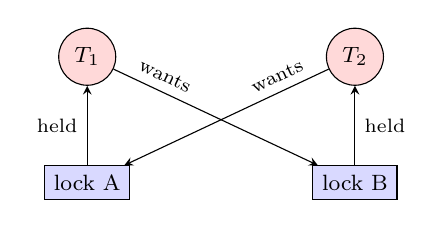
\begin{tikzpicture}[font=\footnotesize, >=stealth, x=1cm, y=1cm]
  \node[draw, circle, fill=red!15] (t1) at (0,1.6) {$T_1$};
  \node[draw, circle, fill=red!15] (t2) at (3.4,1.6) {$T_2$};
  \node[draw, rectangle, fill=blue!15] (la) at (0,0) {lock A};
  \node[draw, rectangle, fill=blue!15] (lb) at (3.4,0) {lock B};
  \draw[->] (t1) -- (lb) node[pos=0.22,above,sloped]{\scriptsize wants};
  \draw[->] (t2) -- (la) node[pos=0.22,above,sloped]{\scriptsize wants};
  \draw[->] (la) -- (t1) node[midway,left]{\scriptsize held};
  \draw[->] (lb) -- (t2) node[midway,right]{\scriptsize held};
\end{tikzpicture}
\caption{The wait-for graph of a textbook deadlock: $T_1$ holds A,
wants B; $T_2$ holds B, wants A. A cycle in this graph is a
deadlock --- and a global lock \emph{order} is what prevents cycles
from ever forming.}
\label{fig:deadlock13}
\end{figure}


Picture two people meeting in a corridor too narrow to pass, each
refusing to step back until the other does. Neither is slow or
broken; each is waiting for the other. A deadlock is that situation
for locks: thread 1 holds A and wants B, thread 2 holds B and wants A.
A deadlock is a cycle in the wait-for graph. Preventing cycles is
simpler than finding them: impose a global lock \emph{order} (always
acquire A before B) and cycles become impossible. Lock-free designs
skip locks entirely but pay in memory-ordering reasoning --- the
[hard] exercise below repairs a broken one informally.

\begin{example}[Make a deadlock happen on purpose, then prevent it]
\emph{What goes wrong first.} Thread 1 locks A then B; thread 2
locks B then A. We put a 0.1\,s sleep between each thread's two
acquisitions so that both always hold their first lock before asking
for the second, which turns a ``rare'' bug into a certain one. A
normal \texttt{pthread\_mutex\_lock} would hang forever, so the demo
uses \texttt{pthread\_mutex\_timedlock} with a one-second limit to
report the stuck state and exit.

\begin{lstlisting}[basicstyle=\ttfamily\scriptsize,caption={Real output of
\texttt{ch13\_deadlock bad} and \texttt{ch13\_deadlock good}. The two
report lines may print in either order.}]
$ ./ch13_deadlock bad
T1: holds A, waited 1 s for B -> deadlock
T2: holds B, waited 1 s for A -> deadlock
opposite order: 2 thread(s) stuck
$ ./ch13_deadlock good
T1: got both locks
T2: got both locks
global order: 0 thread(s) stuck
\end{lstlisting}
The cure is a rule, not cleverness: every thread takes A before B.
Then no thread can hold B while waiting for A, so the cycle cannot
form. The cost is that every programmer must follow the order, which
is why large programs write the order down.
\end{example}

\section{What concurrency actually buys}
\label{sec:amdahl13}

\begin{figure}[htbp]
\centering
\begin{tabular}{lrrr}
\toprule
parallel fraction & speedup @4T & @8T & @$\infty$ \\
\midrule
0.90 & 3.08 & 4.71 & 10.0 \\
0.95 & 3.48 & 5.93 & 20.0 \\
0.99 & 3.88 & 7.48 & 100.0 \\
\bottomrule
\end{tabular}
\caption{Amdahl's arithmetic: at 90\% parallel, 8 cores buy 4.7$\times$,
not 8. The serial 10\% is the ceiling --- which is why the
partitioned counter's flat curve matters more than any lock trick.}
\label{fig:amdahl13}
\end{figure}


At 90\% parallel work, 8 cores buy 4.7$\times$, not 8 --- and the
padded counters' flat curve (167--180\,ms at 1, 2 and 4 threads in
Figure~\ref{fig:falseshare13}) shows the actual path to the
speedup: eliminate the shared state, not just the locks around it.
Amdahl isn't pessimism; it's the design brief.

\section{Common mistakes}
\label{sec:mistakes13}
\begin{itemize}
\item \textbf{``It works on my machine'' races.} The same unfixed
      program lost 29\% to 83\% of its updates across runs here;
      timing and contention decide how visible the bug is, not
      whether it exists.
\item \textbf{Trusting a flat line.} The ``partitioned'' counter
      looked free because gcc turned the loop into one add. A
      measurement better than the hardware allows is a bug in the
      measurement.
\item \textbf{\texttt{if} instead of \texttt{while} on a CV.} Mesa
      semantics require re-checking; the intermittent failure is
      the classic heisenbug.
\item \textbf{Atomic = fast (or slow), assumed.} On the Mac one
      contended line out-cost a mutex at 8 threads; on the Linux
      container the atomic won at every count. Contention is the
      enemy, not the mechanism, and the winner depends on the
      machine.
\item \textbf{Deadlock by ``it can't happen here''}. Any lock
      acquired while holding another can cycle; ordering is
      cheap, analysis is expensive.
\item \textbf{Sharing the cache line, not the data.} Adjacent
      counters on one line bounce between cores (false sharing) ---
      ch10's geometry returning through the abstraction.
\end{itemize}

\section{Summary}
\label{sec:summary13}
\begin{tabularx}{\linewidth}{@{}l X@{}}
\toprule
\textbf{Piece} & \textbf{Verified version} \\
\midrule
race      & 6 threads: 2.48M of 3M updates lost, real \\
atomics   & lr/sc + amo are the hardware's indivisible unit \\
mutex     & scales to 35ms at 8T --- parking cost is real \\
atomic add & Mac: slower than mutex at 8T; Linux container: faster at every count \\
partition & eliminate sharing, not locking; pad counters (adjacent: $2.2\times$ slower at 4T) \\
CV        & \texttt{while}-loop re-check is mandatory \\
Amdahl    & 8T at 90\% parallel = 4.7$\times$, the serial ceiling \\
\bottomrule
\end{tabularx}

\section*{Further reading}
\label{sec:further13}
\begin{itemize}
\item OSTEP ch26--33 (the bug taxonomy and all the classic code):
      \url{https://pages.cs.wisc.edu/~remzi/OSTEP/}
\item xv6 ch6, ch9 (spinlock + sleep/wakeup on a real kernel):
      \url{https://github.com/mit-pdos/xv6-riscv}
\item CS:APP ch12 (concurrent programming):\ \url{https://csapp.cs.cmu.edu/}
\item RISC-V A-extension spec (lr/sc semantics): \texttt{riscv.org/specifications}
\end{itemize}

\begin{rulebox}[Watch instead]
\begin{itemize}
\item \textbf{Concurrency \& Race Conditions --- Computerphile}
      --- the same lost-update demo at this altitude
      (verified 2026-10-11).
      \url{https://youtu.be/7ENFeb-J75k}
\end{itemize}
\end{rulebox}

\section*{Notes}
\label{sec:notes13}
\begin{itemize}
\item The older numbers are verbatim outputs of the chapter's C
      programs on Apple Silicon with clang+pthreads (the atomic-at-8T
      regression is a measured result there). New listings are from a
      Linux x86\_64 container and are labelled. The partition column
      of \texttt{ch13\_lockscale.c} times thread start-up only (the
      loop is optimised away, verified on Linux); the honest
      measurement is \texttt{ch13\_partition.c}.
\item The deliberate-race demo is intentionally volatile-marked ---
      with optimisation and few threads it sometimes ``passes'';
      that unreliability is itself a Common-mistakes entry.
\end{itemize}

\section*{Exercises}
\addcontentsline{toc}{section}{Exercises}
\stepcounter{section}

\begin{exercise}[easy]
Why does the race \emph{sometimes} produce the right answer? Name
the two factors that decide whether the interleaving bites.
\end{exercise}
\begin{solution}[hint]
Timing (how often threads overlap the load-store window) and
contention level; correctness never depends on them, only speed.
\end{solution}

\begin{exercise}[easy]
Distinguish a data race from a race condition in one sentence each.
\end{exercise}
\begin{solution}[hint]
Race: two accesses to one location, one a write, unsynchronised.
Condition: program output depends on interleaving order.
\end{solution}

\begin{exercise}[easy]
What does the mutex actually \emph{do} when it can't acquire the
lock --- on this implementation, sleep or spin?
\end{exercise}
\begin{solution}[hint]
pthreads mutexes park the thread in the kernel; pure spinlocks
burn cycles instead.
\end{solution}

\begin{exercise}[easy]
Why does partitioning beat even an uncontended lock? One line.
\end{exercise}
\begin{solution}[hint]
No shared line means no coherency traffic at all.
\end{solution}

\begin{exercise}[medium]
Show the exact two-instruction interleaving that loses an update in
\texttt{counter++} on a single core. Can it happen on one core?
\end{exercise}
\begin{solution}[hint]
Load 5, preempted; other thread loads 5, stores 6; first stores 6
--- yes, preemption alone suffices.
\end{solution}

\begin{exercise}[medium]
Implement the producer--consumer queue with CVs, then break it by
changing \texttt{while} to \texttt{if}. Describe the failure mode
and why it passes light testing.
\end{exercise}
\begin{solution}[hint]
Two consumers wake on one signal; loser pops empty --- rare under
low load, common at capacity.
\end{solution}

\begin{exercise}[medium]
On the Mac the atomic counter lost to the mutex at 8 threads; on
the Linux container it won at every thread count. Give a cache-terms
explanation for the Mac result and one hypothesis for why it does not
reproduce, and say what you would measure to test it.
\end{exercise}
\begin{solution}[hint]
Every atomic op forces the line to move to the executing core; a
parked thread makes no traffic at all. Hypotheses: different cores,
interconnect and lock implementations. To test, compare hardware
cache-miss counters or sweep the thread count on both machines.
Only a measurement settles it.
\end{solution}

\begin{exercise}[medium]
Design the experiment that distinguishes spinlock vs mutex on a
load where the critical section is 5 instructions. Predict the
crossover point.
\end{exercise}
\begin{solution}[hint]
Sweep contention; spin wins when wait $<$ park/wake cost ---
roughly microseconds.
\end{solution}

\begin{exercise}[medium]
A team replaces a mutex with a lock-free queue and sees latency
\emph{worse} at 2 threads. Two plausible mechanisms?
\end{exercise}
\begin{solution}[hint]
Retry storms under contention, and memory-ordering fences costing
more than the lock's fast path.
\end{solution}

\begin{exercise}[hard]
Prove or repair this ``lock-free'' counter: both writers run a
shared check-then-store on one variable. Give the Dekker-style
argument for the failure, state the ordering assumption used, then
write the correct primitive in pseudo-code.
\end{exercise}
\begin{solution}[hint]
Check-then-act is two operations; need CAS (compare-and-swap) as
one atomic unit --- on RISC-V, lr/sc loop.
\end{solution}

\begin{exercise}[hard]
Extend the lockscale measurement to \emph{reader}-heavy workloads
(95\% reads). Which mechanism wins then, and which C++17/Rust
primitive implements it? Why does it beat a mutex?
\end{exercise}
\begin{solution}[hint]
A shared lock (rwlock/shared\_mutex) wins: read paths don't
serialise; the mutex treats reads as writes.
\end{solution}

\begin{exercise}[hard]
The assembly listing shows the partition loop collapsed to one add.
Predict roughly what the partition column of \texttt{ch13\_lockscale}
would show if \texttt{part} were \texttt{volatile}, using
\texttt{ch13\_partition.c}'s padded timing as your per-increment cost.
\end{exercise}
\begin{solution}[hint]
The padded run does 100\,M increments in about 167\,ms, i.e.\ 1.67\,ns
each. So 400\,000 increments cost about $400000\times1.67\,\text{ns}
\approx0.67$\,ms per thread, against the 0.1\,ms the compiler-deleted
loop reported: roughly $6\times$ higher (more if adjacent counters
share a line).
\end{solution}

\begin{exercise}[easy]
What is the wait-for graph, and which of its shapes is a deadlock?
\end{exercise}
\begin{solution}[hint]
Nodes = threads/locks, edges = holds/wants; a cycle is deadlock.
\end{solution}

\begin{exercise}[medium]
Rank the three fixes by engineering cost: partitioned counter,
mutex, lock-free CAS loop. Which requires the most reasoning per
line of code?
\end{exercise}
\begin{solution}[hint]
Lock-free --- memory ordering is where the real cost lives.
\end{solution}

\begin{exercise}[medium]
False sharing: two threads increment \emph{different} counters on
one cache line. Predict the scaling curve vs truly-private counters
and name the fix.
\end{exercise}
\begin{solution}[hint]
Slower than private counters: measured here, adjacent counters took
$1.8\times$ (2 threads) and $2.2\times$ (4 threads) as long as padded
ones; the fix is to pad each counter to its own 64-byte line.
\end{solution}

\begin{exercise}[easy]
In \texttt{ch13\_prodcons}, the \texttt{while} version reported zero
empty-queue wakeups. Explain why this is guaranteed rather
than lucky.
\end{exercise}
\begin{solution}[hint]
The \texttt{while} test is re-run after every wakeup while holding
the lock, so a consumer proceeds only when the queue is non-empty (or
\texttt{done}). No other thread can change the queue between the test
and the pop because the lock is held.
\end{solution}

\begin{exercise}[medium]
Change \texttt{ch13\_deadlock bad} so that thread 2 takes A first
but keep the sleeps. Predict the output, then say which of the four
deadlock conditions (mutual exclusion, hold-and-wait, no preemption,
circular wait) you removed.
\end{exercise}
\begin{solution}[hint]
Both threads now lock A then B; the second simply waits for the first
to finish, so the output is the ``good'' output (0 stuck). You removed
circular wait; the other three conditions still hold.
\end{solution}
